\subsection{Interleave}
Pour diminuer les effets NUMA, nous pouvons utiliser la politique d'allocation interleave.
%
Cette politique va distribuer équitablement les pages mémoires sur les différents bancs NUMA.
%
Nous allons donc augmenter la bande passante mémoire en ne modifiant que légèrement la latence mémoire moyenne.
%
Sur Rostand, nous obtenons un gain de performance mais toujours pas les même performances qu'en mémoire partagée.
%% TODO résultat manumanu


%   (-_-)   %
\begin{figure}[t!]
  \centering
  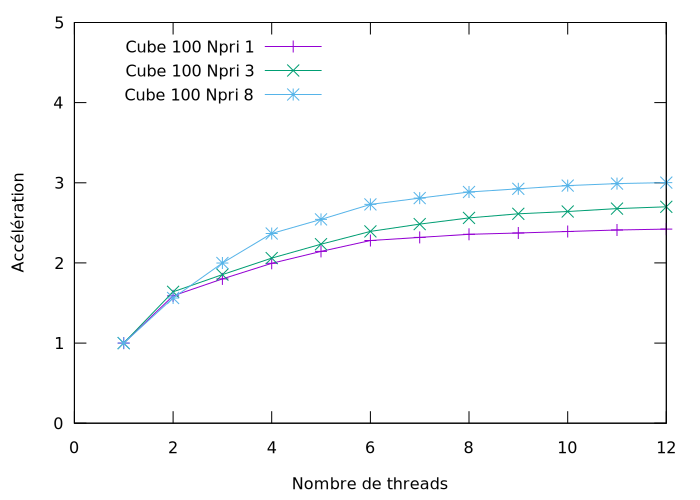
\includegraphics[width=0.7\textwidth]{res_spmv_interleave}
  \caption{Accélération du produit matrice vecteur creux sur Rostand en mémoire partagée avec une politique d'allocation interleave}
  \label{fig:res_spmv_interleave_rostand}
\end{figure}
